%----------------------------------------------------------------------------------------
%    PACKAGES AND THEMES
%----------------------------------------------------------------------------------------
\documentclass[handout, aspectratio=169,xcolor=dvipsnames]{beamer}
\makeatletter
\def\input@path{{theme/}}
\makeatother
\usetheme{CleanEasy}
\usepackage[utf8]{inputenc}
\usepackage{lmodern}
\usepackage[T1]{fontenc}
% \usepackage[brazil]{babel}
\usepackage{fix-cm}
\usepackage{amsmath}
\usepackage{mathtools}
\usepackage{listings}
\usepackage{xcolor}
\usepackage{hyperref}
\usepackage{graphicx} % Allows including images
\usepackage{booktabs} % Allows the use of \toprule, \midrule and \bottomrule in tables
\usepackage{tikz}
\usetikzlibrary{positioning, shapes, arrows, calc, decorations.pathreplacing, arrows.meta, backgrounds, patterns, overlay-beamer-styles}
\usepackage{etoolbox}
\usepackage{animate}
\usepackage{multimedia}
\usepackage{media9}

\usepackage{subfiles}


\newcommand{\bx}{\mathbf{x}}
\newcommand{\by}{\mathbf{y}}
\newcommand{\pd}{p_\text{data}}
\newcommand{\pt}{p_\theta}
\newcommand{\nbx}{\nabla_{\bx}}

\newcommand{\btx}{\mathbf{\tilde{x}}}
\newcommand{\qs}{q_{\sigma}}
\newcommand{\nbtx}{\nabla_{\btx}}

%----------------------------------------------------------------------------------------
%    LAYOUT CONFIGURATION
%----------------------------------------------------------------------------------------
\input{configs/configs}
%----------------------------------------------------------------------------------------

% References from references.bib
\usepackage[backend=bibtex,sorting=none]{biblatex}
\addbibresource{references.bib}


\begin{document}

\section{Week 3}

\begin{frame}{Overview}
\begin{itemize}
    \item Simplified Lorentz Group Equivariant Block (LGEB) from \cite{gongEfficientLorentzEquivariant2022}
    \item Stack layers to turn random noise + time embedding into time-dependent vector field with optimal transport flow matching objective
    \item Produce 30 particles with Cartesian 4-momenta $(p_x, p_y, p_z, E/c)$
\end{itemize}
\end{frame}

\begin{frame}{Modified architecture based on LorentzNet}

    $x$ = Cartesian particle 4-momenta, $\phi_\cdot$ = learnable functions, $\psi(\cdot) = \text{sgn}(\cdot) \log(|\cdot| + 1)$, $c = $ hyperparameter, $N = \#$ particles, $|| \cdot ||, \langle \cdot \rangle$ = Minkowski norm and inner product
    \vspace{0.5cm}
    \begin{columns}
        \begin{column}{0.5\textwidth}
            \textbf{LGEB (\cite{gongEfficientLorentzEquivariant2022})}
            \begin{align*}
                m_{ij}^l &= \phi_e(h_i^l, h_j^l, \psi(||x_i^l - x_j^l||), \psi(\langle x_i^l, x_j^l \rangle)) \\
                m_{ij}^l &= \phi_m(m_{ij}^l) \cdot m_{ij}^l
            \end{align*}
            \begin{align*}
                x_i^{l+1} &= x_i^l + \frac{c}{N} \sum\limits_{j \in [N]} \phi_x(m_{ij}^l) \cdot |x_i - x_j|         
            \end{align*}
            \begin{align*}
                h_i^{l+1} &= h_i^l + \phi_h(h_i^l, \sum\limits_{j \in [N]} \phi_w(m_{ij}^l) m_{ij}^l)
            \end{align*}
        \end{column}
        \begin{column}{0.5\textwidth}
            \textbf{Simple LE block this week}
            \begin{align*}
                m^l_{ij} &= \phi_e(\psi(||x_i^l - x_j^l||), \psi(\langle x_i^l, x_j^l \rangle))\\
                m^l_{ij} &= \phi_m(m^l_{ij}) \cdot m^l_{ij}
            \end{align*}
            \begin{align*}
                x_i^{l+1} &= x_i^l + \frac{c}{N} \sum\limits_{j \in [N]} \phi_x(m_{ij}, g) \cdot |x_j^l - x_i^l|
            \end{align*}
            $g = $ global feature vector (currently time embedding $\phi_t(t)$)
        \end{column}
    \end{columns}
\end{frame}


\begin{frame}{Current architecture}
    \begin{figure}
        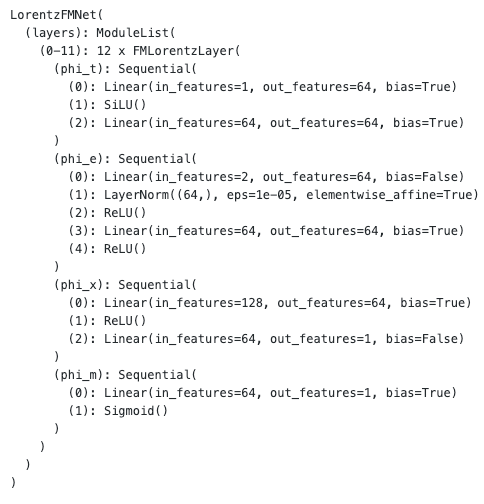
\includegraphics[height=\textheight]{figs/current-architecture.png}
    \end{figure}
\end{frame}

\begin{frame}{Current hyperparameters}
    \begin{itemize}
        \item 12 layers in the model; sample initial noise from Gaussian
        \item Train with conditional optimal transport objective \begin{equation*}
            \mathbb{E}_{t \sim \mathcal{U}[0, 1], q(x_1) \sim \mathcal{J}, p(x_0) \sim \mathcal{N}(0, 1)} || v_t(\phi_t(x_0)) - (x_1 - x_0) ||^2
        \end{equation*}
        \item 1,000 epochs over batches of size 256
        \item Adam opstimizer with learning rate $10^{-3}$
        \item Trained on 124076 gluon jets to avoid zero-padding issue
        \item Generate 50,000 jets with 30 particles each with 16 Euler integration steps
    \end{itemize}
\end{frame}

\begin{frame}{Unit conversion}
    \begin{itemize}
        \item Converted relative particle coordinates $\eta^\text{rel}$, $\phi^\text{rel}$, $p_T^\text{rel}$ to Cartesian $p_x, p_y, p_z, E/c$
        \item Sampled jet $\phi$ values from $\mathcal{U}[0, 2\pi]$
        \item 
    \end{itemize}
\end{frame}

\begin{frame}{Training status}
    \begin{itemize}
        \item Couldn't provision resources on NRP Nautilus in time - had issues creating a custom Dockerfile
        \item Should be done by end of today - just using the base CUDA + Torch dockerfile with install instructions in the Pod YAML
    \end{itemize}
\end{frame}

\begin{frame}{Required work}
    \begin{enumerate}
        \item Feature processing and normalization in Cartesian coordinates
        \item Particle cloud size is currently fixed at 30. Try zero-padding approach like in MPGAN \cite{kansalParticleCloudGeneration2022}, FPCD \cite{mikuniFastPointCloud2023}: sample jet size and ignore masked particles in message-passing steps, ignore in output
        \item Experimentally confirm LE by applying boosts to inputs
    \end{enumerate}
\end{frame}

\begin{frame}{Possible next steps}
    \begin{enumerate}
        \item Global feature vector: \begin{itemize}
            \item If training on all jet types: include type in embedding (\cite{leighFasterDiffusionModel2024})
            \item Condition on global jet features (e.g., jet mass, $p_T$, etc.) (\cite{leighPCJeDiDiffusionParticle2024,kachJetFlowGeneratingJets2022,mikuniFastPointCloud2023,leighFasterDiffusionModel2024,buhmannEPiClyFastParticle2023}). Train NFs to produce base features if necessary for unconditional inference; or try joint training (like in FPCD \cite{mikuniFastPointCloud2023})
            \item Richer time embeddings (e.g., sinusoidal embeddings) (like in FPCD \cite{mikuniFastPointCloud2023})
            \item Include global feature vector in message-passing step
            \item Update global features after each layer (like in EPiC-GAN \cite{buhmannEPiCGANEquivariantPoint2023})
        \end{itemize}
        \item Proof for equivariant output (vector field) $\to$ equivariant probability densities (like in EquiFM \cite{songEquivariantFlowMatching2023})
        \item FM hyperparameters: objectives (eg. variance-preserving, variance-exploding), number of steps, noise scheduler
        % \item Distillation (used in FPCD \cite{mikuniFastPointCloud2023}) / consistency models (used in EPiC-FM \cite{leighFasterDiffusionModel2024}) to improve inference speed 
    \end{enumerate}
\end{frame}

% \begin{frame}{Simulation-based inference}
%     \begin{itemize}
%         \item 
%     \end{itemize}
% \end{frame}

\begin{frame}[allowframebreaks]{References}
\printbibliography
\end{frame}
\end{document}
